\documentclass[preview]{standalone}

% tikz
\usepackage{tikz}
\usetikzlibrary{intersections, angles, quotes, positioning}
\usetikzlibrary{arrows.meta}
\usepackage{pgfplots}
\pgfplotsset{compat=1.13}
\tikzset{
	force/.style={thick, {Circle[length=2pt]}-stealth, shorten <=-1pt}
}

\begin{document}
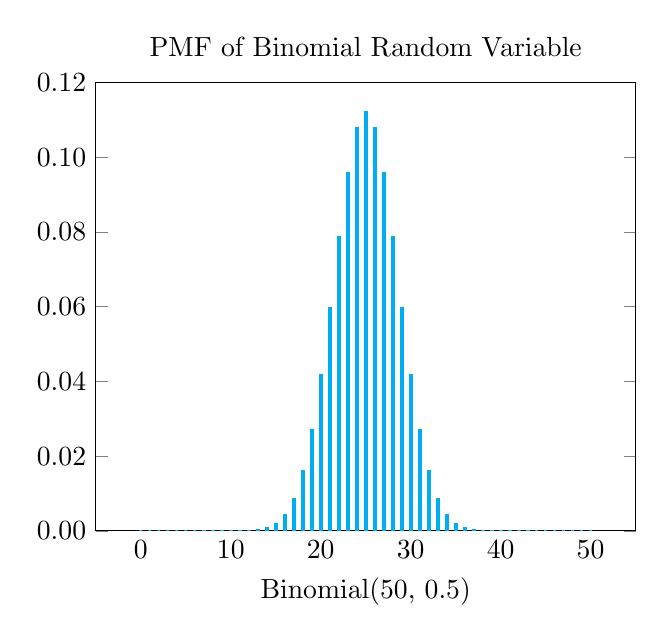
\begin{tikzpicture}
  \begin{axis}
  [
      % Define probability distribution functions
      declare function={
          binom(\n,\p) = \n!/(x!*(\n-x)!)*\p^x*(1-\p)^(\n-x);
          normal(\m,\s) = 1/(\s*sqrt(2*pi))*exp(-((x-\m)^2)/(2*\s^2));
      },
      % Plotting options
      title=PMF of Binomial Random Variable,
      ymin=0,
      ymax=0.12,
      xlabel={Binomial(50, 0.5)},
      samples at={0,...,50},
      xtick style={draw=none},
      yticklabel style={
          /pgf/number format/fixed,
          /pgf/number format/fixed zerofill,
          /pgf/number format/precision=2,
      },   
  ]
  
  % Plot Binomial Distribution
  \addplot [ybar=0pt,bar width=1pt,fill=cyan,draw=cyan] {binom(50,0.5)};
  \end{axis}
  \end{tikzpicture}
\end{document}